\chapter{Results}

    In this chapter we present the results of experiments conducted and provide answers to all research questions from Section~\ref{sec:RQs}. Section~\ref{sec:results_rq1} takes up the majority of this chapter and will be addressing results achieved on the task of \emph{Expertise Extraction}. Analysis results of \emph{Cross-Platform Expertise} will be presented in Section~\ref{sec:results_rq2}, while \emph{Cross-Platform Transferable Knowledge} results will be addressed in Section~\ref{sec:results_rq3}. This chapter will conclude with Section~\ref{sec:results_rq4}, in which we will present our results and conclusions for \emph{Expertise Evolution}.

    \section{Expertise Extraction\label{sec:results_rq1}}
        % RQ1: How to extract the major expertise areas of Stack Overflow and GitHub users? How do expertise trends compare on Stack Overflow and GitHub?
        
        For the \emph{Expertise Extraction} task \emph{3 novel techniques} have been proposed: Topic Distribution based Expertise Extraction \emph{(Technique 1)}, Expertise Extraction using LDA based User and Topic Embeddings \emph{(Technique 2)}, and Expertise Extraction using Pre-trained Word2Vec based User and Topic Embeddings \emph{(Technique 3)}. Techniques 2 and 3 have two different variations each: the first one using \emph{Average-pooling}, while the second one using \emph{Max-pooling} technique for down-sampling. Including these two variations, a total of 5 models are considered:
        
        \begin{itemize}
            \item Model 1: Topic Distribution based Expertise Extraction, labelled Technique \textbf{1} 
            \item Model 2: Expertise Extraction using LDA based User and Topic Embeddings obtained by Average-pooling, labelled in tables as Technique \textbf{2A}  
            \item Model 3: Expertise Extraction using LDA based User and Topic Embeddings obtained by Max-pooling, labelled in tables as Technique \textbf{2B}  
            \item Model 4: Expertise Extraction using Pre-trained Word2Vec based User and Topic Embeddings obtained by Average-pooling, labelled in tables as Technique \textbf{3A} 
            \item Model 5: Expertise Extraction using Pre-trained Word2Vec based User and Topic Embeddings obtained by Max-pooling, labelled in tables as Technique \textbf{3B} 
        \end{itemize}
        
        The above listed 5 models are evaluated against a baseline (naive) model (see Section~\ref{subsec:random_model}), which is a frequency based random model. When evaluating the extraction of expertise areas, two similar experiments were used. In the first experiment each model's performance is evaluated against the ground truth knowledge from section \ref{sec:expertise_survey} with the specification that a model has to output exactly as many expertise terms as the ground truth annotation contains. This case is referred to as \emph{Experiment 1}. In the second experiment each model is evaluated against the ground truth annotation, but there are no restrictions applied to the number of expertise terms to be returned by each model. In this scenario the models can be more robust, as they can return all the expertise terms found by the underlying algorithm, without needing to rank and return only the top-$n$ expertise terms. Throughout this chapter this more robust, less restrictive experiment setup will be referred to as \emph{Experiment 2}. Furthermore, each one of the above mentioned experiments has to variations: expertise extraction from i.) GitHub data (labelled \emph{Experiment} \textbf{A}) and ii.) Stack Overflow data (labelled \emph{Experiment} \textbf{B}).
        
        \begin{table}
          \centering
          \caption{Results of Experiment 1A - Expertise Extraction from GitHub data}\label{tab:GH_results1}
            \vspace{6pt} % Required to get proper spacing between caption and table
          \begin{tabular}{|c|c|c|c|c|c|c|c|}
            \hline
            \thead{Top 3\\Results}& \diaghead{\theadfont DiagonalHead}{Metrics}{Model} &
            \thead{Topic Distr.\\based (\textbf{1})} & \thead{LDA based\\(\textbf{2A})} & \thead{LDA based\\(\textbf{2B})} & \thead{Word2Vec\\based (\textbf{3A})} & \thead{Word2Vec\\based (\textbf{3B})} & \thead{Random\\(\textbf{Baseline})} \\
            \hline
            \multirow{3}*{1} & Cosine Sim. & 0.6690 & 0.7187 & 0.7357 & \textbf{0.7998} & 0.7317 & 0.5962 \\
                  & Jaccard Sim. & 0.0658 & 0.0751 & 0.1040 & 0.0765 & 0.1049 & 0.0286 \\
                  & BLEU Score & 0.1197 & 0.1340 & 0.1767 & 0.1368 & 0.1782 & 0.0540 \\
            \hline
            \multirow{3}*{2} & Cosine Sim. & 0.6689 & 0.7183 & 0.7351 & 0.7959 & 0.7316 & 0.5962 \\
                   & Jaccard Sim. & 0.0658 & 0.0750 & 0.1037 & 0.0818 & 0.1049 & 0.0286 \\
                   & BLEU Score & 0.1197 & 0.1338 & 0.1762 & 0.1452 & 0.1782 & 0.0540 \\
            \hline
            \multirow{3}*{3} & Cosine Sim. & 0.6683 & 0.7183 & 0.7351 & 0.7959 & 0.7316 & 0.5962 \\
                   & Jaccard Sim. & 0.0652 & 0.750 & 0.1037 & 0.0818 & 0.1049 & 0.0286 \\
                   & BLEU Score & 0.1186 & 0.1338 & 0.1762 & 0.1452 & 0.1782 & 0.0540 \\
          \hline 
        \end{tabular}
        \end{table}
        
        
        
        \begin{table}
            \centering
          \caption{Parameters of Models from Experiment 1A - Expertise Extraction from GitHub data}\label{tab:GH_params1}
            \vspace{6pt} % Required to get proper spacing between caption and table
          \begin{tabular}{|c|c|c|c|c|c|c|}
            \hline
            \thead{Top 3\\Results}& \diaghead{\theadfont DiagonalHead}{Parameters}{Model} &
            \thead{Topic Distr.\\based (\textbf{1})} & \thead{LDA based\\(\textbf{2A})} & \thead{LDA based \\(\textbf{2B})} & \thead{Word2Vec\\based (\textbf{3A})} & \thead{Word2Vec\\based (\textbf{3B})}\\
            \hline
            \multirow{3}*{1} & Topic Number & 11 & 10 & 11 & \textbf{16} & 11 \\
                  & Beta Value & 0.01 & 0.005 & 0.05 & \textbf{0.05} & 0.05 \\
                  & Threshold & X & X & X & \textbf{X} & X \\
            \hline
            \multirow{3}*{2} & Topic Number & 11 & 10 & 11 & 16 & 11 \\
                   & Beta Value & 0.005 & 0.001 & 0.001 & 0.001 & 0.001 \\
                   & Threshold & X & X & X & X & X \\
            \hline
            \multirow{3}*{3} & Topic Number & 11 & 10 & 11 & 16 & 11 \\
                   & Beta Value & 0.05 & 0.01 & 0.005 & 0.005 & 0.005 \\
                   & Threshold & X & X & X & X & X \\
          \hline 
        \end{tabular}
        \end{table}
        
        
        
        \begin{table}
          \centering
          \caption{Results of Experiment 1B - Expertise Extraction from Stack Overflow data} \label{tab:SO_results1}
            \vspace{6pt} % Required to get proper spacing between caption and table
          \begin{tabular}{|c|c|c|c|c|c|c|c|}
            \hline
            \thead{Top 3\\Results}& \diaghead{\theadfont DiagonalHead}{Metrics}{Model} &
            \thead{Topic Distr.\\based (\textbf{1})} & \thead{LDA based\\(\textbf{2A})} & \thead{LDA based \\(\textbf{2B})} & \thead{Word2Vec\\based (\textbf{3A})} & \thead{Word2Vec\\based (\textbf{3B})} & \thead{Random\\(\textbf{Baseline})}\\
            \hline
            \multirow{3}*{1} & Cosine Sim. & 0.5044 & 0.5582 & \textbf{0.5837} & 0.5607 & 0.5820 & 0.3721 \\
                  & Jaccard Sim. & 0.016 & 0.0406 & 0.0435 & 0.0320 & 0.0556 & 0.0104 \\
                  & BLEU Score & 0.0313 & 0.0770 & 0.0823 & 0.0612 & 0.1041 & 0.0199 \\
            \hline
            \multirow{3}*{2} & Cosine Sim. & 0.4997 & 0.5560 & 0.5717 & 0.5574 & 0.5746 & 0.3721 \\
                  & Jaccard Sim. & 0.0295 & 0.0747 & 0.0814 & 0.0404 & 0.0784 & 0.0104 \\
                  & BLEU Score & 0.0560 & 0.1366 & 0.1471 & 0.0768 & 0.1424 & 0.0199 \\
            \hline
            \multirow{3}*{3} & Cosine Sim. & 0.4755 & 0.5409 & 0.5676 & 0.5537 & 0.5736 & 0.3721 \\
                  & Jaccard Sim. & 0.0127 & 0.0754 & 0.0821 & 0.0718 & 0.0305 & 0.0104 \\
                  & BLEU Score & 0.0247 & 0.1366 & 0.1478 & 0.1312 & 0.0584 & 0.0199 \\
          \hline 
        \end{tabular}
        \end{table}
        
        
        
        \begin{table}
            \centering
          \caption{Parameters of Models from Experiment 1B - Expertise Extraction from Stack Overflow data} \label{tab:SO_params1}
            \vspace{6pt} % Required to get proper spacing between caption and table
          \begin{tabular}{|c|c|c|c|c|c|c|}
            \hline
            \thead{Top 3\\Results}& \diaghead{\theadfont Diagonal Head}{Parameter}{Model} &
            \thead{Topic Distr.\\based (\textbf{1})} & \thead{LDA based\\(\textbf{2A})} & \thead{LDA based \\(\textbf{2B})} & \thead{Word2Vec\\based (\textbf{3A})} & \thead{Word2Vec\\based (\textbf{3B})}\\
            \hline
            \multirow{3}*{1} & Topic Number & 40 & 33 & \textbf{33} & 31 & 48 \\
                  & Beta Value & 0.01 & 1 & \textbf{1} & 0.1 & 1 \\
                  & Threshold & X & X & \textbf{X} & X & X \\
            \hline
            \multirow{3}*{2} & Topic Number & 29 & 27 & 27 & 48 & 27 \\
                   & Beta Value & 0.1 & 0.5 & 0.5 & 1 & 1 \\
                   & Threshold & X & X & X & X & X \\
            \hline
            \multirow{3}*{3} & Topic Number & 45 & 16 & 27 & 14 & 31 \\
                   & Beta Value & 0.1 & 0.5 & 1 & 1 & 1 \\
                   & Threshold & X & X & X & X & X \\
          \hline 
        \end{tabular}
        \end{table}
        
        \begin{table}
              \centering
              \caption{Example of Cosine Similarity Scores between Word-Pairs} \label{tab:SO_LDA_labels}
                \vspace{6pt} % Required to get proper spacing between caption and table
              \begin{tabular}{|c c c|c c c|}
                \hline
                Word 1 & Word 2 & Cosine Similarity & Word 1 & Word 2 & Cosine Similarity \\
                \hline
                php & reactjs & 0.1499 & css & html & 0.5631 \\
                php & python & 0.2529 & c & c++ & 0.6177 \\
                java & python & 0.3929 & tensorflow & sklearn & 0.6858 \\ 
                analysis & visualization & 0.4524 & mysql & postgresql & 0.7997 \\
                nodejs & reactjs & 0.4909 & keras & tensorflow & 0.8391 \\
                \hline
              \end{tabular}
            \end{table}
        
        \subsection{GitHub and Stack Overflow Topic Patterns}
            
            \begin{table}
              \centering
              \caption{Labels given to topics of the best LDA model trained on Stack Overflow}\label{tab:SO_LDA_labels}
                \vspace{6pt} % Required to get proper spacing between caption and table
              \begin{tabular}{|c|c|c|c|c|c|}
                \hline
                Topic & Given Name & Topic & Given Name & Topic & Given Name \\
                \hline
                1 & & 12 & & 23 &  \\
                2 & & 13 & & 24 &  \\
                3 & & 14 & & 25 &  \\
                4 & & 15 & & 26 &  \\
                5 & & 16 & & 27 &  \\
                6 & & 17 & & 28 &  \\
                7 & & 18 & & 29 &  \\
                8 & & 19 & & 30 &  \\
                9 & & 20 & & 31 &  \\
                10 & & 21 & & 32 &  \\
                11 & & 22 & & 33 &  \\
                \hline
              \end{tabular}
            \end{table}
            
            \begin{table}
              \centering
              \caption{Labels given to topics of the best LDA model trained on GitHub}\label{tab:GH_LDA_labels}
                \vspace{6pt} % Required to get proper spacing between caption and table
              \begin{tabular}{|c|c|c|c|}
                \hline
                Topic & Given Name & Topic & Given Name \\
                \hline
                1 & & 9 &  \\
                2 & & 10 &  \\
                3 & & 11 &  \\
                4 & & 12 &  \\
                5 & & 13 &  \\
                6 & & 14 &  \\
                7 & & 15 &  \\
                8 & & 16 &  \\
                \hline
              \end{tabular}
            \end{table}
        
        \boxed{$Answer to RQ1:$}
    
    \section{Cross-platform Expertise\label{sec:results_rq2}}
        %RQ2: How similar are developer expertise profiles in two different collaborator platforms, Stack Overflow and GitHub?

        \begin{figure}
          % Requires 
          \centering
          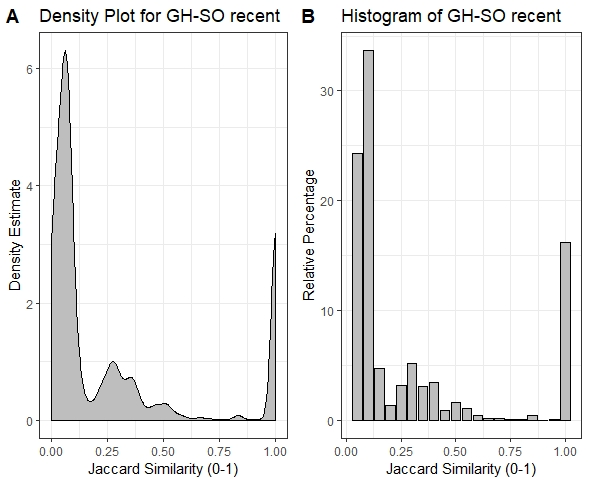
\includegraphics[width=\textwidth]{figures/GH_SO_recent.jpeg}\\
          \caption{Density Plot(A) and Histogram(B) of GH-recent and SO-recent data set comparison}
          \label{fig:GH_SO_recent}
        \end{figure}
        
        \begin{figure}
          % Requires 
          \centering
          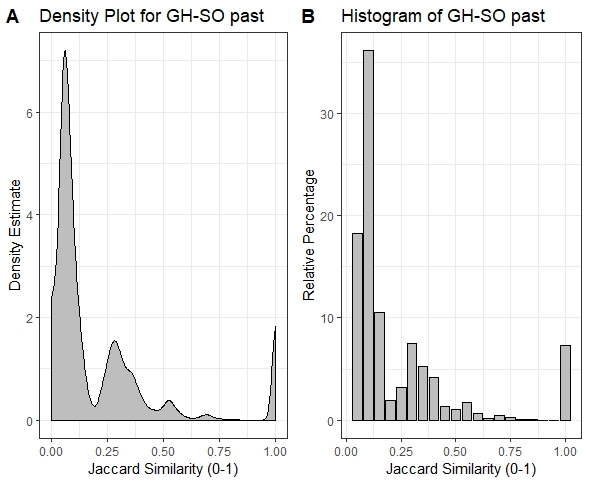
\includegraphics[width=\textwidth]{figures/GH_SO_past.jpeg}\\
          \caption{Density Plot(A) and Histogram(B) of GH-past and SO-past data set comparison}
          \label{fig:GH_SO_past}
        \end{figure}
        
        
        \begin{figure}
          % Requires 
          \centering
          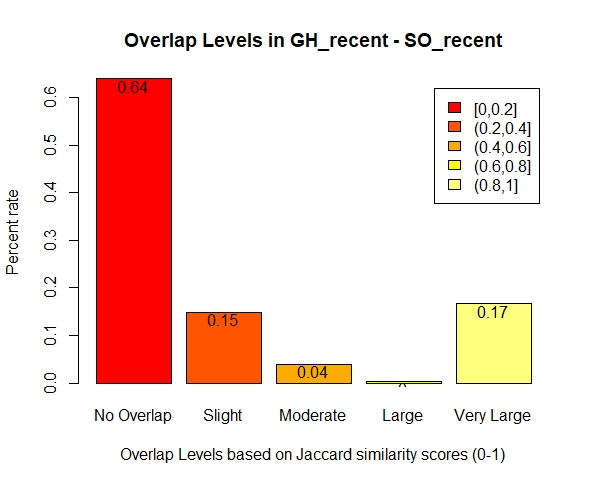
\includegraphics[width=\textwidth]{figures/overlap_GH_SO_recent.jpeg}\\
          \caption{Overlap levels between GH-recent and SO-recent data sets}
          \label{fig:overlap_GH_SO_recent}
        \end{figure}
        
        \begin{figure}
          % Requires 
          \centering
          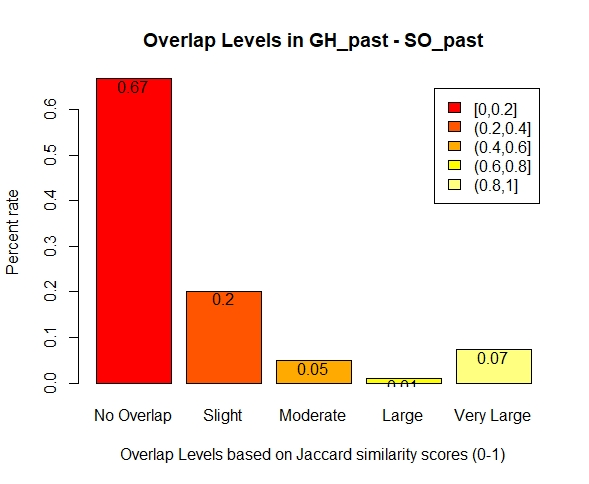
\includegraphics[width=\textwidth]{figures/overlap_SO_GH_past.jpeg}\\
          \caption{Overlap levels between GH-past and SO-past data sets}
          \label{fig:overlap_GH_SO_past}
        \end{figure}
        
        %\fbox{\begin{minipage}{15em}
        %...
        %\end{minipage}}
        
        \boxed{$Answer to RQ2:$}
    
    \section{Cross-platform Transferable Knowledge\label{sec:results_rq3}}
        % RQ3:  What knowledge is transferable from one platform to another?
        
        \begin{table}
          \centering
          \caption{Most common words in GH-past and SO-past data sets.}\label{tab:RQ3_past}
            \vspace{6pt} % Required to get proper spacing between caption and table
          \begin{tabular}{|c c c | c c c|}
            \hline
            Ranking & Keyword & Frequency & Ranking & Keyword & Frequency \\
            \hline\hline
            1 & library & 43123 & 16 & base & 16798 \\
            2 & code & 37621 & 17 & implementation & 16670 \\
            3 & simple & 32762 & 18 & client & 15833 \\
            4 & type & 30948 & 19 & test & 15723 \\
            5 & javascript & 30044 & 20 & http & 15674 \\
            6 & project & 26255 & 21 & page & 15423 \\
            7 & web & 25083 & 22 & game & 13890 \\
            8 & tool & 24967 & 23 & website & 13255 \\
            9 & https & 24738 & 24 & package & 12982 \\
            10 & file & 24737 & 25 & repository & 11690 \\
            11 & html & 22333 & 26 & add & 11421 \\
            12 & github & 21317 & 27 & method & 11421 \\
            13 & script & 20318 & 28 & line & 11252 \\
            14 & source & 20266 & 29 & api & 11144 \\
            15 & language & 19855 & 30 & datum & 10980 \\
            \hline
          \end{tabular}
        \end{table}
        
        
        \begin{table}
          \centering
          \caption{Most common words in GH-recent and SO-recent data sets.}\label{tab:RQ3_recent}
            \vspace{6pt} % Required to get proper spacing between caption and table
          \begin{tabular}{|c c c | c c c|}
            \hline
            Ranking & Keyword & Frequency & Ranking & Keyword & Frequency \\
            \hline\hline
            1 & test & 56302 & 16 & heroku & 15764 \\
            2 & simple & 51226 & 17 & buildpack & 15764 \\
            3 & library & 44781 & 18 & cli & 15764 \\
            4 & app & 43750 & 19 & rb & 15764 \\
            5 & api & 35881 & 20 & activerecord & 15764 \\
            6 & base & 26075 & 21 & rspec & 15764 \\
            7 & client & 25381 & 22 & active & 15764 \\
            8 & code & 22052 & 23 & github & 15297 \\
            9 & file & 21538 & 24 & web & 12890 \\
            10 & application & 19620 & 25 & add & 12849 \\
            11 & https & 16764 & 26 & change & 12849\\
            12 & ruby & 15764  & 27 & remove & 12849 \\
            13 & rail & 15764 & 28 & check & 12849\\
            14 & ember & 15764 & 29 & make & 11231 \\
            15 & gem & 15764 & 30 & comment & 11231\\
            \hline
          \end{tabular}
        \end{table}
        
        Co-occuring keywords: \textbf{test, simple, library, api, base, client, code, file, https, github, web} and \textbf{add}.
        
        \boxed{$Answer to RQ3:$}
    
    \section{Expertise Evolution\label{sec:results_rq4}}
        % RQ4: How does developer expertise evolve on Stack Overflow and GitHub?
                
        \begin{figure}
          % Requires 
          \centering
          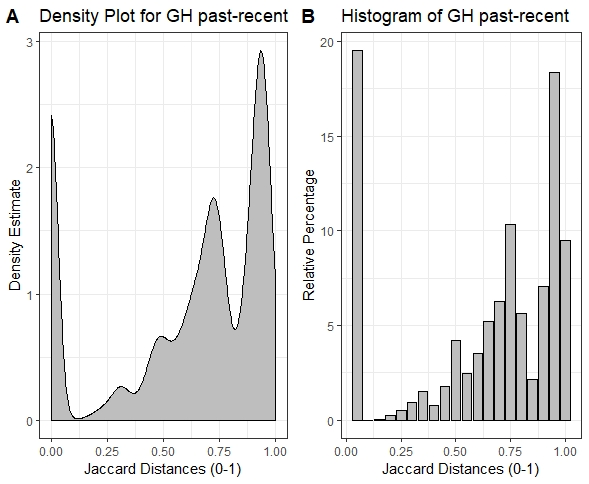
\includegraphics[width=\textwidth]{figures/GH_past-recent.jpeg}\\
          \caption{Density Plot(A) and Histogram(B) of GitHub past and recent data set comparison}
          \label{fig:GH_past_recent}
        \end{figure}
        
        \begin{figure}
          % Requires 
          \centering
          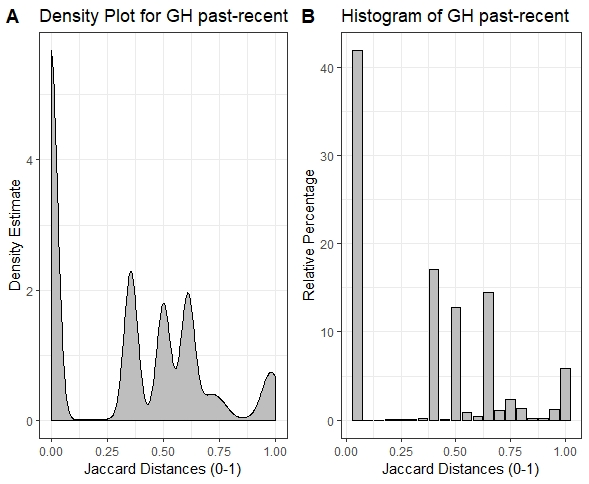
\includegraphics[width=\textwidth]{figures/SO_past-recent.jpeg}\\
          \caption{Density Plot(A) and Histogram(B) of Stack Overflow past and recent data set comparison}
          \label{fig:SO_past_recent}
        \end{figure}
        
        
        \begin{figure}
          % Requires 
          \centering
          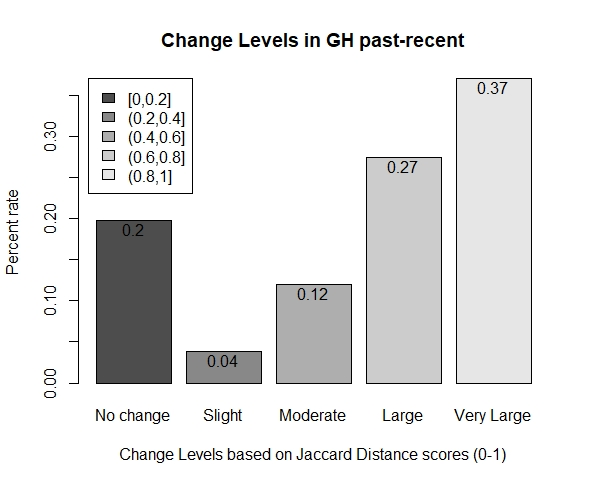
\includegraphics[width=\textwidth]{figures/change_level_GH_past-recent.jpeg}\\
          \caption{Change levels between GitHub past and recent data sets}
          \label{fig:change_GH_past_recent}
        \end{figure}
        
        \begin{figure}
          % Requires 
          \centering
          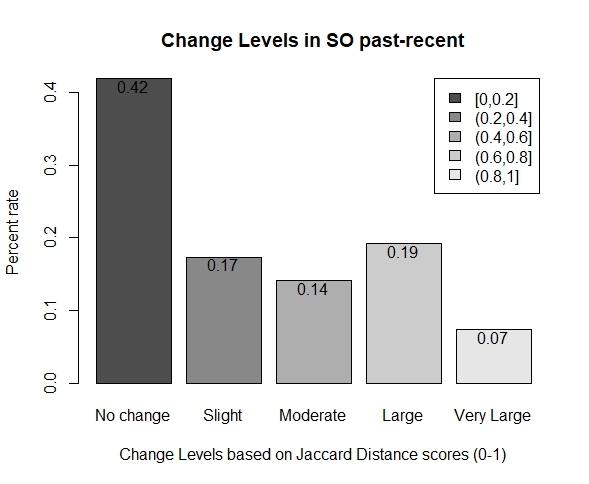
\includegraphics[width=\textwidth]{figures/change_levels_SO_past-recent.jpeg}\\
          \caption{Change levels between Stack Overflow past and recent data sets}
          \label{fig:change_SO_past_recent}
        \end{figure}
        
        \boxed{$Answer to RQ4:$}